%% template.tex
%% from
%% bare_conf.tex
%% V1.4b
%% 2015/08/26
%% by Michael Shell
%% See:
%% http://www.michaelshell.org/
%% for current contact information.
%%
%% This is a skeleton file demonstrating the use of IEEEtran.cls
%% (requires IEEEtran.cls version 1.8b or later) with an IEEE
%% conference paper.
%%
%% Support sites:
%% http://www.michaelshell.org/tex/ieeetran/
%% http://www.ctan.org/pkg/ieeetran
%% and
%% http://www.ieee.org/

%%*************************************************************************
%% Legal Notice:
%% This code is offered as-is without any warranty either expressed or
%% implied; without even the implied warranty of MERCHANTABILITY or
%% FITNESS FOR A PARTICULAR PURPOSE!
%% User assumes all risk.
%% In no event shall the IEEE or any contributor to this code be liable for
%% any damages or losses, including, but not limited to, incidental,
%% consequential, or any other damages, resulting from the use or misuse
%% of any information contained here.
%%
%% All comments are the opinions of their respective authors and are not
%% necessarily endorsed by the IEEE.
%%
%% This work is distributed under the LaTeX Project Public License (LPPL)
%% ( http://www.latex-project.org/ ) version 1.3, and may be freely used,
%% distributed and modified. A copy of the LPPL, version 1.3, is included
%% in the base LaTeX documentation of all distributions of LaTeX released
%% 2003/12/01 or later.
%% Retain all contribution notices and credits.
%% ** Modified files should be clearly indicated as such, including  **
%% ** renaming them and changing author support contact information. **
%%*************************************************************************


% *** Authors should verify (and, if needed, correct) their LaTeX system  ***
% *** with the testflow diagnostic prior to trusting their LaTeX platform ***
% *** with production work. The IEEE's font choices and paper sizes can   ***
% *** trigger bugs that do not appear when using other class files.       ***                          ***
% The testflow support page is at:
% http://www.michaelshell.org/tex/testflow/

\documentclass[conference,final,]{IEEEtran}
% Some Computer Society conferences also require the compsoc mode option,
% but others use the standard conference format.
%
% If IEEEtran.cls has not been installed into the LaTeX system files,
% manually specify the path to it like:
% \documentclass[conference]{../sty/IEEEtran}





% Some very useful LaTeX packages include:
% (uncomment the ones you want to load)


% *** MISC UTILITY PACKAGES ***
%
%\usepackage{ifpdf}
% Heiko Oberdiek's ifpdf.sty is very useful if you need conditional
% compilation based on whether the output is pdf or dvi.
% usage:
% \ifpdf
%   % pdf code
% \else
%   % dvi code
% \fi
% The latest version of ifpdf.sty can be obtained from:
% http://www.ctan.org/pkg/ifpdf
% Also, note that IEEEtran.cls V1.7 and later provides a builtin
% \ifCLASSINFOpdf conditional that works the same way.
% When switching from latex to pdflatex and vice-versa, the compiler may
% have to be run twice to clear warning/error messages.






% *** CITATION PACKAGES ***
%
%\usepackage{cite}
% cite.sty was written by Donald Arseneau
% V1.6 and later of IEEEtran pre-defines the format of the cite.sty package
% \cite{} output to follow that of the IEEE. Loading the cite package will
% result in citation numbers being automatically sorted and properly
% "compressed/ranged". e.g., [1], [9], [2], [7], [5], [6] without using
% cite.sty will become [1], [2], [5]--[7], [9] using cite.sty. cite.sty's
% \cite will automatically add leading space, if needed. Use cite.sty's
% noadjust option (cite.sty V3.8 and later) if you want to turn this off
% such as if a citation ever needs to be enclosed in parenthesis.
% cite.sty is already installed on most LaTeX systems. Be sure and use
% version 5.0 (2009-03-20) and later if using hyperref.sty.
% The latest version can be obtained at:
% http://www.ctan.org/pkg/cite
% The documentation is contained in the cite.sty file itself.






% *** GRAPHICS RELATED PACKAGES ***
%
\ifCLASSINFOpdf
  % \usepackage[pdftex]{graphicx}
  % declare the path(s) where your graphic files are
  % \graphicspath{{../pdf/}{../jpeg/}}
  % and their extensions so you won't have to specify these with
  % every instance of \includegraphics
  % \DeclareGraphicsExtensions{.pdf,.jpeg,.png}
\else
  % or other class option (dvipsone, dvipdf, if not using dvips). graphicx
  % will default to the driver specified in the system graphics.cfg if no
  % driver is specified.
  % \usepackage[dvips]{graphicx}
  % declare the path(s) where your graphic files are
  % \graphicspath{{../eps/}}
  % and their extensions so you won't have to specify these with
  % every instance of \includegraphics
  % \DeclareGraphicsExtensions{.eps}
\fi
% graphicx was written by David Carlisle and Sebastian Rahtz. It is
% required if you want graphics, photos, etc. graphicx.sty is already
% installed on most LaTeX systems. The latest version and documentation
% can be obtained at:
% http://www.ctan.org/pkg/graphicx
% Another good source of documentation is "Using Imported Graphics in
% LaTeX2e" by Keith Reckdahl which can be found at:
% http://www.ctan.org/pkg/epslatex
%
% latex, and pdflatex in dvi mode, support graphics in encapsulated
% postscript (.eps) format. pdflatex in pdf mode supports graphics
% in .pdf, .jpeg, .png and .mps (metapost) formats. Users should ensure
% that all non-photo figures use a vector format (.eps, .pdf, .mps) and
% not a bitmapped formats (.jpeg, .png). The IEEE frowns on bitmapped formats
% which can result in "jaggedy"/blurry rendering of lines and letters as
% well as large increases in file sizes.
%
% You can find documentation about the pdfTeX application at:
% http://www.tug.org/applications/pdftex





% *** MATH PACKAGES ***
%
%\usepackage{amsmath}
% A popular package from the American Mathematical Society that provides
% many useful and powerful commands for dealing with mathematics.
%
% Note that the amsmath package sets \interdisplaylinepenalty to 10000
% thus preventing page breaks from occurring within multiline equations. Use:
%\interdisplaylinepenalty=2500
% after loading amsmath to restore such page breaks as IEEEtran.cls normally
% does. amsmath.sty is already installed on most LaTeX systems. The latest
% version and documentation can be obtained at:
% http://www.ctan.org/pkg/amsmath





% *** SPECIALIZED LIST PACKAGES ***
%
%\usepackage{algorithmic}
% algorithmic.sty was written by Peter Williams and Rogerio Brito.
% This package provides an algorithmic environment fo describing algorithms.
% You can use the algorithmic environment in-text or within a figure
% environment to provide for a floating algorithm. Do NOT use the algorithm
% floating environment provided by algorithm.sty (by the same authors) or
% algorithm2e.sty (by Christophe Fiorio) as the IEEE does not use dedicated
% algorithm float types and packages that provide these will not provide
% correct IEEE style captions. The latest version and documentation of
% algorithmic.sty can be obtained at:
% http://www.ctan.org/pkg/algorithms
% Also of interest may be the (relatively newer and more customizable)
% algorithmicx.sty package by Szasz Janos:
% http://www.ctan.org/pkg/algorithmicx




% *** ALIGNMENT PACKAGES ***
%
%\usepackage{array}
% Frank Mittelbach's and David Carlisle's array.sty patches and improves
% the standard LaTeX2e array and tabular environments to provide better
% appearance and additional user controls. As the default LaTeX2e table
% generation code is lacking to the point of almost being broken with
% respect to the quality of the end results, all users are strongly
% advised to use an enhanced (at the very least that provided by array.sty)
% set of table tools. array.sty is already installed on most systems. The
% latest version and documentation can be obtained at:
% http://www.ctan.org/pkg/array


% IEEEtran contains the IEEEeqnarray family of commands that can be used to
% generate multiline equations as well as matrices, tables, etc., of high
% quality.




% *** SUBFIGURE PACKAGES ***
%\ifCLASSOPTIONcompsoc
%  \usepackage[caption=false,font=normalsize,labelfont=sf,textfont=sf]{subfig}
%\else
%  \usepackage[caption=false,font=footnotesize]{subfig}
%\fi
% subfig.sty, written by Steven Douglas Cochran, is the modern replacement
% for subfigure.sty, the latter of which is no longer maintained and is
% incompatible with some LaTeX packages including fixltx2e. However,
% subfig.sty requires and automatically loads Axel Sommerfeldt's caption.sty
% which will override IEEEtran.cls' handling of captions and this will result
% in non-IEEE style figure/table captions. To prevent this problem, be sure
% and invoke subfig.sty's "caption=false" package option (available since
% subfig.sty version 1.3, 2005/06/28) as this is will preserve IEEEtran.cls
% handling of captions.
% Note that the Computer Society format requires a larger sans serif font
% than the serif footnote size font used in traditional IEEE formatting
% and thus the need to invoke different subfig.sty package options depending
% on whether compsoc mode has been enabled.
%
% The latest version and documentation of subfig.sty can be obtained at:
% http://www.ctan.org/pkg/subfig




% *** FLOAT PACKAGES ***
%

%\usepackage{fixltx2e}
% fixltx2e, the successor to the earlier fix2col.sty, was written by
% Frank Mittelbach and David Carlisle. This package corrects a few problems
% in the LaTeX2e kernel, the most notable of which is that in current
% LaTeX2e releases, the ordering of single and double column floats is not
% guaranteed to be preserved. Thus, an unpatched LaTeX2e can allow a
% single column figure to be placed prior to an earlier double column
% figure.
% Be aware that LaTeX2e kernels dated 2015 and later have fixltx2e.sty's
% corrections already built into the system in which case a warning will
% be issued if an attempt is made to load fixltx2e.sty as it is no longer
% needed.
% The latest version and documentation can be found at:
% http://www.ctan.org/pkg/fixltx2e


%\usepackage{stfloats}
% stfloats.sty was written by Sigitas Tolusis. This package gives LaTeX2e
% the ability to do double column floats at the bottom of the page as well
% as the top. (e.g., "\begin{figure*}[!b]" is not normally possible in
% LaTeX2e). It also provides a command:
%\fnbelowfloat
% to enable the placement of footnotes below bottom floats (the standard
% LaTeX2e kernel puts them above bottom floats). This is an invasive package
% which rewrites many portions of the LaTeX2e float routines. It may not work
% with other packages that modify the LaTeX2e float routines. The latest
% version and documentation can be obtained at:
% http://www.ctan.org/pkg/stfloats
% Do not use the stfloats baselinefloat ability as the IEEE does not allow
% \baselineskip to stretch. Authors submitting work to the IEEE should note
% that the IEEE rarely uses double column equations and that authors should try
% to avoid such use. Do not be tempted to use the cuted.sty or midfloat.sty
% packages (also by Sigitas Tolusis) as the IEEE does not format its papers in
% such ways.
% Do not attempt to use stfloats with fixltx2e as they are incompatible.
% Instead, use Morten Hogholm'a dblfloatfix which combines the features
% of both fixltx2e and stfloats:
%
% \usepackage{dblfloatfix}
% The latest version can be found at:
% http://www.ctan.org/pkg/dblfloatfix




% *** PDF, URL AND HYPERLINK PACKAGES ***
%
%\usepackage{url}
% url.sty was written by Donald Arseneau. It provides better support for
% handling and breaking URLs. url.sty is already installed on most LaTeX
% systems. The latest version and documentation can be obtained at:
% http://www.ctan.org/pkg/url
% Basically, \url{my_url_here}.




% *** Do not adjust lengths that control margins, column widths, etc. ***
% *** Do not use packages that alter fonts (such as pslatex).         ***
% There should be no need to do such things with IEEEtran.cls V1.6 and later.
% (Unless specifically asked to do so by the journal or conference you plan
% to submit to, of course. )



%% BEGIN MY ADDITIONS %%


\usepackage{graphicx}
% We will generate all images so they have a width \maxwidth. This means
% that they will get their normal width if they fit onto the page, but
% are scaled down if they would overflow the margins.
\makeatletter
\def\maxwidth{\ifdim\Gin@nat@width>\linewidth\linewidth
\else\Gin@nat@width\fi}
\makeatother
\let\Oldincludegraphics\includegraphics
\renewcommand{\includegraphics}[1]{\Oldincludegraphics[width=\maxwidth]{#1}}

\usepackage[unicode=true]{hyperref}

\hypersetup{
            pdftitle={Are facial expressions the genuine display of individuals' subjective feeling? A comparison with human and automatic recognition.},
            pdfborder={0 0 0},
            breaklinks=true}
\urlstyle{same}  % don't use monospace font for urls

% Pandoc toggle for numbering sections (defaults to be off)
\setcounter{secnumdepth}{0}

% Pandoc syntax highlighting

% Pandoc header
\usepackage{booktabs}
\usepackage{float}
\usepackage{tabu}

\providecommand{\tightlist}{%
  \setlength{\itemsep}{0pt}\setlength{\parskip}{0pt}}

%% END MY ADDITIONS %%


\hyphenation{op-tical net-works semi-conduc-tor}

\begin{document}
%
% paper title
% Titles are generally capitalized except for words such as a, an, and, as,
% at, but, by, for, in, nor, of, on, or, the, to and up, which are usually
% not capitalized unless they are the first or last word of the title.
% Linebreaks \\ can be used within to get better formatting as desired.
% Do not put math or special symbols in the title.
\title{Are facial expressions the genuine display of individuals' subjective
feeling? A comparison with human and automatic recognition.}

% author names and affiliations
% use a multiple column layout for up to three different
% affiliations

\author{

%% ---- classic IEEETrans wide authors' list ----------------
 % -- end affiliation.wide
%% ----------------------------------------------------------



%% ---- classic IEEETrans one column per institution --------
 %% -- beg if/affiliation.institution-columnar
\IEEEauthorblockN{
  %% -- beg for/affiliation.institution.author
Damien Dupré %% -- end for/affiliation.institution.author
}
\IEEEauthorblockA{Dublin City University\\
Dublin, Ireland
\\damien.dupre@dcu.ie
}
\and
\IEEEauthorblockN{
  %% -- beg for/affiliation.institution.author
Anna Tcherkassof %% -- end for/affiliation.institution.author
}
\IEEEauthorblockA{Grenoble Alpes University\\
Grenoble, France
  %% -- beg for/affiliation.institution.author
\\anna.tcherkassof@univ-grenoble-alpes.fr
 %% -- end for/affiliation.institution.author
}
 %% -- end for/affiliation.institution
 %% -- end if/affiliation.institution-columnar
%% ----------------------------------------------------------





%% ---- one column per author, classic/default IEEETrans ----
 %% -- end if/affiliation.institution-columnar
%% ----------------------------------------------------------

}

% conference papers do not typically use \thanks and this command
% is locked out in conference mode. If really needed, such as for
% the acknowledgment of grants, issue a \IEEEoverridecommandlockouts
% after \documentclass

% for over three affiliations, or if they all won't fit within the width
% of the page, use this alternative format:
%
%\author{\IEEEauthorblockN{Michael Shell\IEEEauthorrefmark{1},
%Homer Simpson\IEEEauthorrefmark{2},
%James Kirk\IEEEauthorrefmark{3},
%Montgomery Scott\IEEEauthorrefmark{3} and
%Eldon Tyrell\IEEEauthorrefmark{4}}
%\IEEEauthorblockA{\IEEEauthorrefmark{1}School of Electrical and Computer Engineering\\
%Georgia Institute of Technology,
%Atlanta, Georgia 30332--0250\\ Email: see http://www.michaelshell.org/contact.html}
%\IEEEauthorblockA{\IEEEauthorrefmark{2}Twentieth Century Fox, Springfield, USA\\
%Email: homer@thesimpsons.com}
%\IEEEauthorblockA{\IEEEauthorrefmark{3}Starfleet Academy, San Francisco, California 96678-2391\\
%Telephone: (800) 555--1212, Fax: (888) 555--1212}
%\IEEEauthorblockA{\IEEEauthorrefmark{4}Tyrell Inc., 123 Replicant Street, Los Angeles, California 90210--4321}}




% use for special paper notices
%\IEEEspecialpapernotice{(Invited Paper)}




% make the title area
\maketitle

% As a general rule, do not put math, special symbols or citations
% in the abstract
\begin{abstract}
While it has been taken for granted in the development of several
automatic facial expression recognition tools, the question of the link
between subjective feelings and facial expressions is still a subject of
debate. On one hand the behaviorist approach conceives emotions as
genetically hardwired and therefore being genuinely displayed through
facial expressions. On the other hand the constructivist approach
conceives emotions are socially constructed and facial expression as
social messages that are not related to emotions. In order to evaluate
the link between the subjective feeling of emotions and their
recognition based on facial expression, 232 videos of participants
recruited to perform an emotion elicitation task were annotated by 1383
human observers as well as by an automatic facial expression classifier.
The results show a low accuracy of human observers and of the automatic
classifier to infer from the facial expression the subjective feeling of
the participants recorded. Based on these results, the hypothesis of
genetically hardwired emotion genuinely display is difficult to support
whereas the idea of emotion socially constructed and facial expression
as display of social messages appears to be more likely. Then, the way
to infer emotional and mental state based on facial expressions should
be questioned.
\end{abstract}

% no keywords

% use for special paper notices



% make the title area
\maketitle

% no keywords

% For peer review papers, you can put extra information on the cover
% page as needed:
% \ifCLASSOPTIONpeerreview
% \begin{center} \bfseries EDICS Category: 3-BBND \end{center}
% \fi
%
% For peerreview papers, this IEEEtran command inserts a page break and
% creates the second title. It will be ignored for other modes.
\IEEEpeerreviewmaketitle


\hypertarget{introduction}{%
\section{Introduction}\label{introduction}}

With the development of commercial automatic facial expression
recognition tools (see Dupré et al. 2018 for a non-exhaustive list of
available tools), industries and governments are gradually implementing
this technology in order to track humans' emotions in various scenarios
(e.g., marketing, healthcare, automotive to name a few). Beside the
ethical question of measuring human emotions, these tools are
challenging psychological theories about inferring emotions from facial
expressions. When automatic facial expression recognition tools are used
to measure human emotions, they rest on the premise that facial
expressions provide a direct access to expressers' emotions. However the
link between emotion felt and facial expressions is far from being
established and still remain a hot topic in psychology research.

\hypertarget{the-link-between-emotion-and-facial-expression-thought-the-behaviorist-approach}{%
\subsection{The link between emotion and facial expression thought the
behaviorist
approach}\label{the-link-between-emotion-and-facial-expression-thought-the-behaviorist-approach}}

Based on the behaviorist approach initiated by Darwin in \emph{The
Expression of the Emotions in Man and Animals} (Darwin 1872), facial
expression are conceived as a genuine display of individuals inner
emotional state. This hypothesis is used as a basis for the Basic
Emotion Theory (BET) which states that a set of six or seven emotions
are universally displayed and are genetically hardwired not only in
humans (Ekman 1992) but also in different animal species (Waal 2019).
According to this view, ``when emotions are aroused by perception of a
social event, a set of central commands produce patterned
emotion-specific changes in multiple systems, including {[}\ldots{}{]}
facial expressions.'' (Ekman 2007, p49). Even if this theory obtained a
popular support, it fails to explain how individuals can feel emotions
without expressing them and how individuals can express emotions without
feeling them.

\hypertarget{the-link-between-emotion-and-facial-expression-thought-the-social-constructivist-approach}{%
\subsection{The link between emotion and facial expression thought the
social constructivist
approach}\label{the-link-between-emotion-and-facial-expression-thought-the-social-constructivist-approach}}

Detractors of the Basic Emotion Theory are perceiving emotion not as
genetically hardwired but as a learnt association between a given
situation and an appropriate response (Averill 1980,
@barrett2017emotions). For the tenants of the constructivist approach,
emotions are ``concepts'' based on past experiences and which are ``a
collection of embodied, whole brain representations that predict what is
about to happen in the sensory environment, what the best action is to
deal with impending events, and their consequences for allostasis''
(Barrett 2017b, p12). Following this assumption, faces are used as tools
to display signals in social interactions (Crivelli and Fridlund 2018).
These signals can convey individuals' motivations and readiness (Frijda
and Tcherkassof 1997) or social messages (Fridlund and Rosenberg 1995).

This current paper investigates the link between the subjective feeling
of emotions and their recognition from facial expressions. If emotions
are hardwired, individuals emotional subjective feeling should be
correlated to the recognition of facial expressions from both human
observers and automatic classifiers whereas if emotions are social
constructs, no correlation between subjective feeling and facial
expression recognition should be observed.

\hypertarget{method}{%
\section{Method}\label{method}}

To evaluate the link between subjective feeling of emotions and their
recognition from facial expressions, participants were recruited to
perform an emotion elicitation task while their facial expression was
video recorded. Then, the videos was shown to human observer and
analysed by an automatic classifier in order to identify which emotion
was displayed.

\hypertarget{emotion-elicitation}{%
\subsection{Emotion Elicitation}\label{emotion-elicitation}}

For the emotion elicitation experiment, 358 French participants (182
females, 176 males, \emph{M}age = 47.9, \emph{SD}age = 9.2) were
recruited to perform one out of 11 emotions elicitation tasks designed
to trigger a positive, negative or neutral emotional state (see
Tcherkassof et al. 2013 for a description of tasks and procedure).
Participants' face were recorded using an hidden camera resulting 358
front facing 768x576 videos varying from 1s to 1479s.

After their emotion elicitation task the participants had to rate their
emotional state during the task on a likert scale from 0 (``not at
all'') to 5 (``strongly'') the six ``basic'' emotions (i.e.,
\emph{anger}, \emph{disgust}, \emph{fear}, \emph{happiness},
\emph{surprise} and \emph{sadness}) as well as six ``non-basic''
emotions (i.e., \emph{pride}, \emph{curiosity}, \emph{boredom},
\emph{shame}, \emph{humiliation}, and \emph{disappointment}).

Finally, a debriefing session was perform to ensure that participants
were not durably affected by the emotion elicitation task. All the
participants gave their agreement on their data and video to be
processed for research purpose only.

\hypertarget{human-facial-expression-recognition}{%
\subsection{Human Facial Expression
Recognition}\label{human-facial-expression-recognition}}

For the human facial expression recognition method, 1383 student
participants were recruited to annotate 232 out of the 358 video,
therefore only the 232 annotated videos will be analysed in this paper.
Each participants had to annotate between 1 and 177 videos resulting
that each video was annotated 29 times on average (\emph{SD} = 12).

The annotation of facial expressions was performed on-site using
\emph{Oudjat}, a software for designing video annotation experiments
(Dupré et al. 2015). For each video, the annotation procedure hat two
steps. First, the participants had to identify the emotional sequences
by pressing the space bar of their keyboard to indicate the beginning
and the end of the emotional sequences while watching the video. Second,
the participants watched each emotional sequence previously identified
and had to label the sequence using one of the 12 emotions proposed
including six ``basic'' emotions (i.e., \emph{anger}, \emph{disgust},
\emph{fear}, \emph{happiness}, \emph{surprise} and \emph{sadness}) and
six ``non-basic'' emotions (i.e., \emph{pride}, \emph{curiosity},
\emph{boredom}, \emph{shame}, \emph{humiliation}, and
\emph{disappointment}). They also had the possibility to indicate that
the sequence was not expressing one of the proposed emotion.

This annotation procedure results in a uni-dimensional time-series for
each video per human observer identifying for each second of the video
which emotion was recognized. Then time-series corresponding to the same
video were aggregated to calculate the proportion of human observers for
each second of the video per emotional label. The sum of each label
proportion per second was used as a score to determine which labels
corresponds to the overall video (i.e., the highest score). In case of
more than one label having the maximum value, the emotion is described
as undetermined.

\hypertarget{automatic-facial-expression-recognition}{%
\subsection{Automatic Facial Expression
Recognition}\label{automatic-facial-expression-recognition}}

The 232 annotated video were processed with Affdex (SDK v3.4.1). Affdex
is an automatic facial expression recognition classifier developed and
distributed by Affectiva is a spin-off company resulting from the
research activities of MIT media lab created in 2009 (McDuff et al.
2016). Affdex's algorithm uses Histogram of Oriented Gradient (HOG)
features and Support Vector Machine (SVM) classifiers in order to
recognize facial expressions. For each video frame, Affdex identify the
probability of the face as expressing one of the six ``basic'' emotions
(i.e., \emph{anger}, \emph{disgust}, \emph{fear}, \emph{happiness},
\emph{surprise} and \emph{sadness}) as well as additional psychological
states such as \emph{valence}, \emph{engagement} or \emph{contempt}, and
facial features such as \emph{cheek raise}, \emph{eye widen} or
\emph{jaw drop}.

To determine which of the six ``basic'' emotion can be used to identify
each video, the recognition probability for each label by frame was
converted into odd ratio by frame (Dente et al. 2017). The highest sum
of each odd ratio time-series defines the label recognized by the
automatic classifier.

\hypertarget{results}{%
\section{Results}\label{results}}

Whereas the self-reports, the human annotations and the automatic
recognition include data on ``non-basic'' emotions and features, the
analysis is performed using only the six ``basic'' emotions in order to
compare them. The maximum score for self-reports, human annotations and
automatic recognition is used to label the video. In case of more than
one label obtaining the maximum value, the video is labeled as
undetermined.

\hypertarget{correlation-between-self-report-and-human-facial-expression-recognition}{%
\subsection{Correlation between self-report and human facial expression
recognition}\label{correlation-between-self-report-and-human-facial-expression-recognition}}

Emotions self-reported as being characteristic of the elicitation are
compared with the emotion recognized by the human observers in a
confusion matrix (Figure \ref{fig:confusionMatrix_sr_hr}).

\begin{figure}
\centering
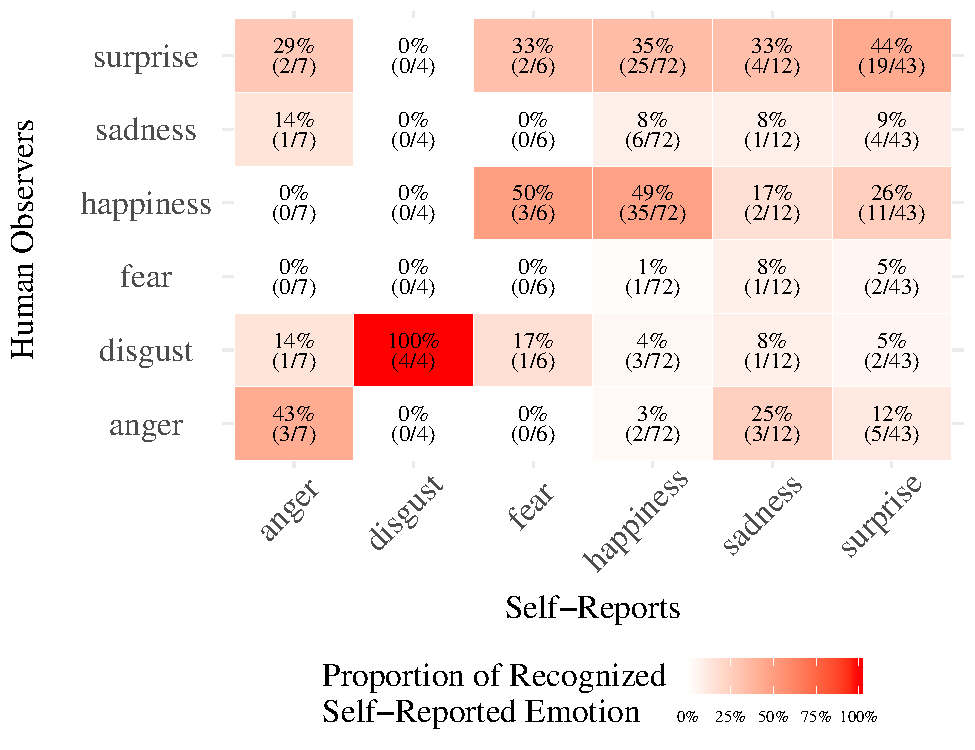
\includegraphics{ACII_2019_paper_files/figure-latex/confusionMatrix_sr_hr-1.pdf}
\caption{Confusion matrix of between the emotion self-reported as being
characteristic of the elicitation with the emotion recognized by the
human observers.}
\end{figure}

The result of the confusion matrix show a low agreement between emotion
felt during the elicitation and emotion recognized by the human
annotators (Accuracy = 0.27, 95\%CI{[}0.21,0.33{]}; Kappa = 0.11) except
for \emph{happiness} (15.2\%), \emph{surprise} (8.26\%) and
\emph{disgust} (1.74\%). Sensitivity, specificity, precision and F1
score for each emotion can be found Table
\ref{tab:confusionTable_sr_hr}. Interestingly human annotators seem to
recognize as \emph{surprise} videos in which \emph{happiness} was the
highest self-reported emotion (10.9\%), and in a lower instance
\emph{happiness} videos in which \emph{surprise} was the highest
self-reported emotion (4.78\%).

\begin{table}[!h]

\caption{\label{tab:confusionTable_sr_hr}Agreement accuracy metrics for each emotion. }
\centering
\fontsize{8}{10}\selectfont
\begin{tabu} to \linewidth {>{\raggedright}X>{\centering}X>{\centering}X>{\centering}X>{\centering}X}
\toprule
Emotion & Sensitivity & Specificity & Precision & F1\\
\midrule
anger & 0.43 & 0.92 & 0.14 & 0.21\\
disgust & 1.00 & 0.93 & 0.20 & 0.33\\
fear & 0.00 & 0.96 & 0.00 & \textit{na.}\\
happiness & 0.49 & 0.73 & 0.45 & 0.47\\
sadness & 0.08 & 0.91 & 0.05 & 0.06\\
surprise & 0.44 & 0.67 & 0.23 & 0.31\\
undetermined & 0.00 & 0.99 & 0.00 & \textit{na.}\\
\bottomrule
\multicolumn{5}{l}{\textsuperscript{} Note. \textit{na.} values are produced when not enough}\\
\multicolumn{5}{l}{data are available to compute accuracy indicators.}\\
\end{tabu}
\end{table}

However, the self-report show a very high proportion of undetermined
emotional states which reveals not only the possibility of the emotion
elicitation tasks to trigger more than one emotion but also the
potential limit of using 6-points likert scales for which the
participants can easily score to the maximum for more than one emotion.

\hypertarget{correlation-between-self-report-and-automatic-facial-expression-recognition}{%
\subsection{Correlation between self-report and automatic facial
expression
recognition}\label{correlation-between-self-report-and-automatic-facial-expression-recognition}}

As in the previous analysis, emotions self-reported as being
characteristic of the elicitation are compared with the emotion
recognized by the automatic classifier in a confusion matrix (Figure
\ref{fig:confusionMatrix_sr_ar}).

\begin{figure}
\centering
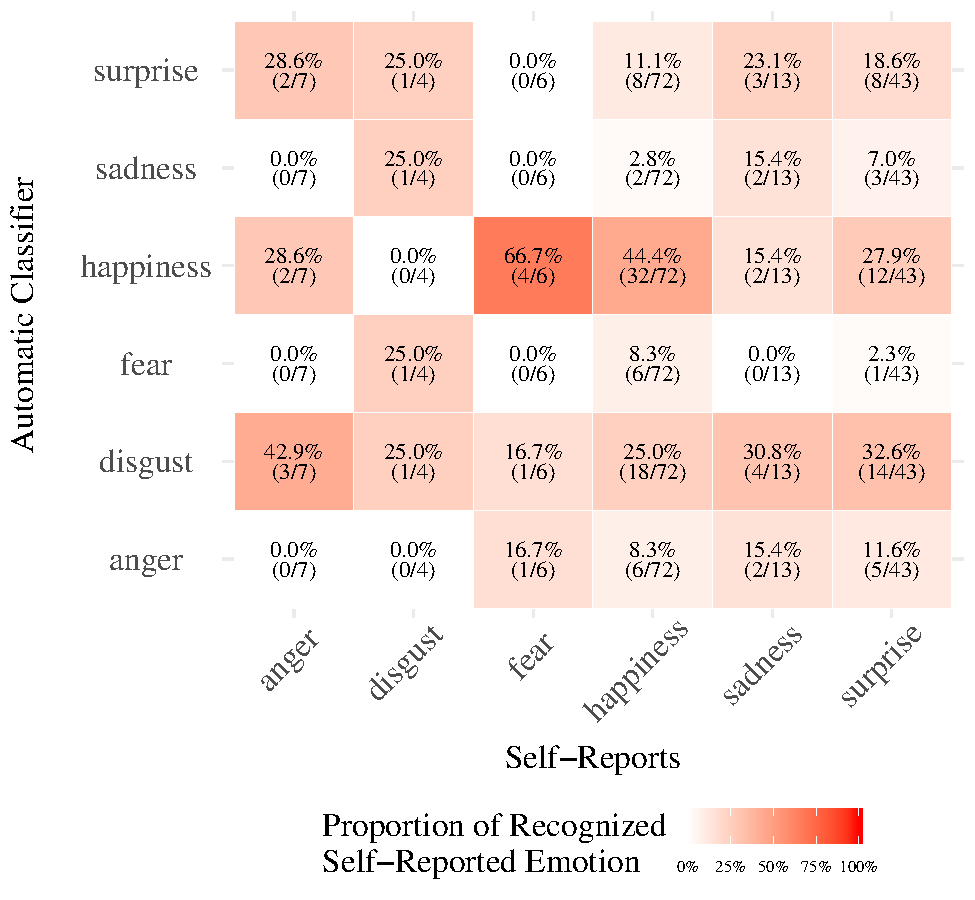
\includegraphics{ACII_2019_paper_files/figure-latex/confusionMatrix_sr_ar-1.pdf}
\caption{Confusion matrix of between the emotion self-reported as being
characteristic of the elicitation with the emotion recognized by the
automatic classifier.}
\end{figure}

Results obtained for the comparison between emotions self-reported and
recognized by the automatic classifier are similar to the ones with
human observers (Table \ref{tab:confusionTable_sr_ar}). Overall there is
a low agreement between emotion self-reported and emotion recognized by
the automatic classifier (Accuracy = 0.19, 95\%CI{[}0.14,0.24{]}; Kappa
= 0.05) except for \emph{happiness} (13.9\%) and \emph{surprise}
(3.48\%). Surprisingly the automatic classifier incorrectly recognized
as \emph{disgust} an important proportion of videos in which
\emph{happiness} was the highest self-reported emotion (7.83\%). In
parallel, the automatic classifier recognized as \emph{happiness} and
\emph{disgust} videos in which \emph{surprise} was the highest
self-reported emotion (respectively 5.22\% and 6.09\%).

\begin{table}[!h]

\caption{\label{tab:confusionTable_sr_ar}Agreement accuracy metrics for each emotion.}
\centering
\fontsize{8}{10}\selectfont
\begin{tabu} to \linewidth {>{\raggedright}X>{\centering}X>{\centering}X>{\centering}X>{\centering}X}
\toprule
Emotion & Sensitivity & Specificity & Precision & F1\\
\midrule
anger & 0.00 & 0.89 & 0 & \textit{na.}\\
disgust & 0.25 & 0.70 & 0.01 & 0.03\\
fear & 0.00 & 0.93 & 0 & \textit{na.}\\
happiness & 0.44 & 0.71 & 0.41 & 0.43\\
sadness & 0.15 & 0.94 & 0.14 & 0.15\\
surprise & 0.19 & 0.89 & 0.28 & 0.22\\
undetermined & 0.00 & 1.00 & \textit{na.} & \textit{na.}\\
\bottomrule
\multicolumn{5}{l}{\textsuperscript{} Note. \textit{na.} values are produced when not enough data are}\\
\multicolumn{5}{l}{available to compute accuracy indicators.}\\
\end{tabu}
\end{table}

A comparable explanation can be provided as the level of undetermined
emotion are very high for the self reports.

\hypertarget{comparison-between-human-and-automatic-recognition}{%
\subsection{Comparison between human and automatic
recognition}\label{comparison-between-human-and-automatic-recognition}}

As previously mentioned, the accuracy of humans observers and the
automatic classifier have some similarities. In order to compare which
recognition has the highest accuracy a Receiver Operating Characteristic
(ROC) curve was calculated (Figure \ref{fig:roc}).

\begin{figure}
\centering
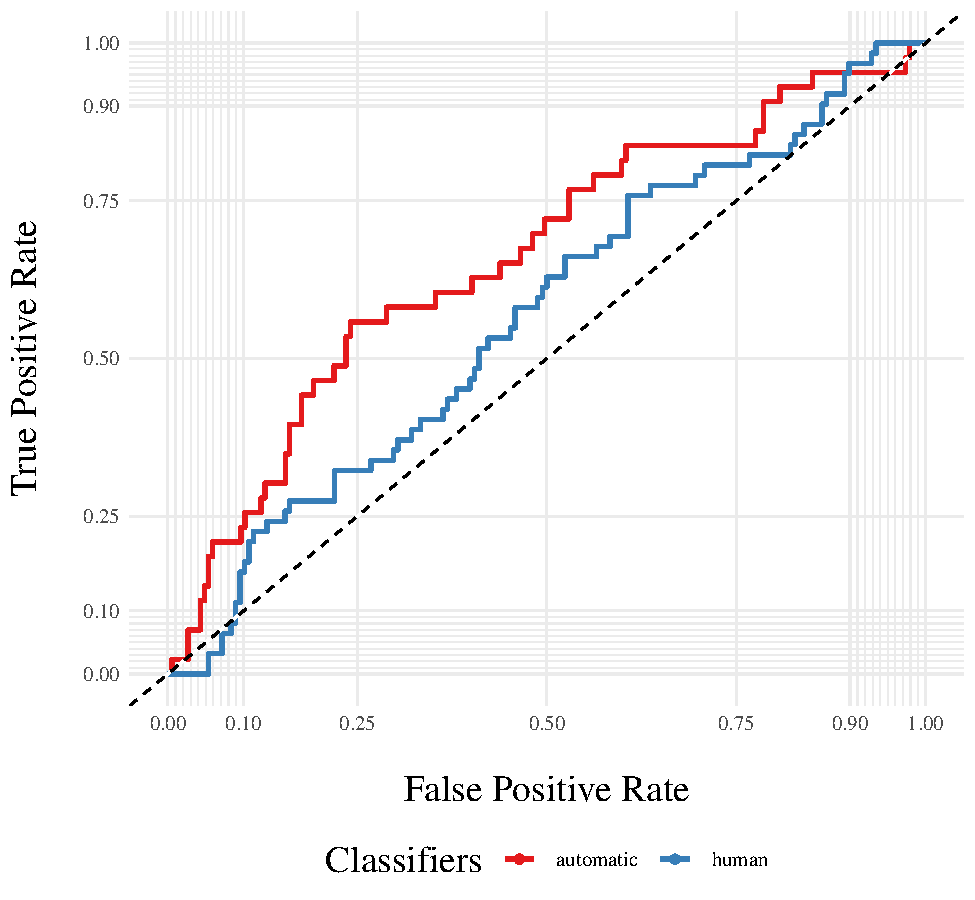
\includegraphics{ACII_2019_paper_files/figure-latex/roc-1.pdf}
\caption{ROC curve comparing the accuracy in inferring subjective
feelings from facial expressions by human observers and automatic
recognition.}
\end{figure}

The ROC curve and its Area Under the Curve (AUC) values shows that the
automatic classifier are more accurate than human observers in inferring
subjective feeling from facial expressions (human AUC = 0.57 \emph{vs.}
automatic AUC = 0.66).

\hypertarget{conclusion}{%
\section{Conclusion}\label{conclusion}}

Despite being one on the most investigated question in affective
science, the link between emotion felt and facial expression is a hot
topic and no clear evidence have been found to definitely answer it.
However, with the growing interest of industries and government to
monitor individual's psychological states, evidences are showing that
facial expressions are in reality not expressing emotions (McKeown
2013). This research aimed to provide some empirical data to the
question. The subjective feeling of participants was compared with human
recognition on one side and automatic recognition on the other side. The
results reveals a low accuracy for both humans and automatic classifier
to accurately identify the inner emotional states of these individuals
based on their facial expressions.

Some limitations to this process should be stated over the use of
self-reports to evaluate individual's subjective feelings. Accessing to
the inner subjective feeling can be biased if not impossible. Moreover
the laboratory setting can trigger ambiguous and ``non-basic'' emotions
which were not analysed in this research. The procedure use for human
annotation can also be incriminated. Instead of asking the human
annotators to provide an unique label, a more subtle approach was chosen
to mimic results provided by the automatic classifier. In this regard,
the results of the human annotation could have been more ambiguous
because it is not the natural way that people are inferring human
emotions. Finally, the automatic classifier algorithm can also be
problematic. Based on training datasets which are most of the time using
prototypical facial expression of the ``basic'' emotions, the algorithm
to classify facial expressions can be held in check by the spontaneous
facial expressions analysed.

Considering the above, the results provides an additional evidence that
individuals' subjective feeling can not be inferred from facial
expressions and in our case invalidate the hypothesis of hardwired
emotions. This result suggests that automatic facial expression
recognition tools should be focused on evaluating facial morphology
features such as action units rather than inferring potential emotional
or affective states.

\hypertarget{acknowledgment}{%
\section{Acknowledgment}\label{acknowledgment}}

The authors would like to thank Brigitte Meillon and Jean Michel Adam
who developed the software used to collect and preprocess human observer
annotations.

\hypertarget{references}{%
\section*{References}\label{references}}
\addcontentsline{toc}{section}{References}

\hypertarget{refs}{}
\leavevmode\hypertarget{ref-averill1980constructivist}{}%
Averill, James R. 1980. ``A Constructivist View of Emotion.'' In
\emph{Theories of Emotion}, 305--39. Elsevier.

\leavevmode\hypertarget{ref-barrett2017emotions}{}%
Barrett, Lisa Feldman. 2017a. \emph{How Emotions Are Made: The Secret
Life of the Brain}. Houghton Mifflin Harcourt.

\leavevmode\hypertarget{ref-barrett2017theory}{}%
---------. 2017b. ``The Theory of Constructed Emotion: An Active
Inference Account of Interoception and Categorization.'' \emph{Social
Cognitive and Affective Neuroscience} 12 (1): 1--23.

\leavevmode\hypertarget{ref-crivelli2018facial}{}%
Crivelli, Carlos, and Alan J Fridlund. 2018. ``Facial Displays Are Tools
for Social Influence.'' \emph{Trends in Cognitive Sciences} 22 (5):
388--99.

\leavevmode\hypertarget{ref-darwin1872expression}{}%
Darwin, Charles. 1872. \emph{The Expression of the Emotions in Man and
Animals}. London, UK: John Murray, London UK.

\leavevmode\hypertarget{ref-dente2017measures}{}%
Dente, Pasquale, Dennis Küster, Lina Skora, and E Krumhuber. 2017.
``Measures and Metrics for Automatic Emotion Classification via Facet.''
In \emph{Proceedings of the Conference on the Study of Artificial
Intelligence and Simulation of Behaviour (Aisb)}, 160--63.

\leavevmode\hypertarget{ref-dupre2015oudjat}{}%
Dupré, Damien, Daniel Akpan, Elena Elias, Jean-Michel Adam, Brigitte
Meillon, Nicolas Bonnefond, Michel Dubois, and Anna Tcherkassof. 2015.
``Oudjat: A Configurable and Usable Annotation Tool for the Study of
Facial Expressions of Emotion.'' \emph{International Journal of
Human-Computer Studies} 83: 51--61.

\leavevmode\hypertarget{ref-dupre2018accuracy}{}%
Dupré, Damien, Nicole Andelic, Gawain Morrison, and Gary McKeown. 2018.
``Accuracy of Three Commercial Automatic Emotion Recognition Systems
Across Different Individuals and Their Facial Expressions.'' In
\emph{2018 Ieee International Conference on Pervasive Computing and
Communications Workshops (Percom Workshops)}, 627--32. IEEE.

\leavevmode\hypertarget{ref-ekman1992argument}{}%
Ekman, Paul. 1992. ``An Argument for Basic Emotions.'' \emph{Cognition
\& Emotion} 6 (3-4): 169--200.

\leavevmode\hypertarget{ref-ekman2007directed}{}%
---------. 2007. ``The Directed Facial Action Task.'' \emph{Handbook of
Emotion Elicitation and Assessment} 47: 53.

\leavevmode\hypertarget{ref-fridlund1995human}{}%
Fridlund, Alan J, and Erika L Rosenberg. 1995. ``Human Facial
Expression: An Evolutionary View.'' \emph{Nature} 373 (6515): 569--69.

\leavevmode\hypertarget{ref-frijda1997facial}{}%
Frijda, Nico H, and Anna Tcherkassof. 1997. ``Facial Expressions as
Modes of Action Readiness.'' \emph{The Psychology of Facial Expression},
78--102.

\leavevmode\hypertarget{ref-mcduff2016affdex}{}%
McDuff, Daniel, Abdelrahman Mahmoud, Mohammad Mavadati, May Amr, Jay
Turcot, and Rana el Kaliouby. 2016. ``AFFDEX Sdk: A Cross-Platform
Real-Time Multi-Face Expression Recognition Toolkit.'' In
\emph{Proceedings of the 2016 Chi Conference Extended Abstracts on Human
Factors in Computing Systems}, 3723--6. ACM.

\leavevmode\hypertarget{ref-mckeown2013analogical}{}%
McKeown, Gary J. 2013. ``The Analogical Peacock Hypothesis: The Sexual
Selection of Mind-Reading and Relational Cognition in Human
Communication.'' \emph{Review of General Psychology} 17 (3): 267--87.

\leavevmode\hypertarget{ref-tcherkassof2013dynemo}{}%
Tcherkassof, Anna, Damien Dupré, Brigitte Meillon, Nadine Mandran,
Michel Dubois, and Jean-Michel Adam. 2013. ``DynEmo: A Video Database of
Natural Facial Expressions of Emotions.'' \emph{The International
Journal of Multimedia \& Its Applications} 5 (5): 61--80.

\leavevmode\hypertarget{ref-de2019mama}{}%
Waal, Frans de. 2019. \emph{Mama's Last Hug: Animal Emotions and What
They Teach Us About Ourselves}. Granta Books.

\end{document}


